\documentclass[11pt, addpoints, answers]{exam}

\usepackage{amsmath, amssymb, amsthm, euler}
\usepackage{xcolor}
\usepackage{tikz}

% headers, footers, titles
\newcommand{\CourseName}{CS101 Algorithms and Data Structures}
\newcommand{\HomeworkNO}{Homework 11}
\newcommand{\DueDate}{Due date: 23:59, December 11th, 2022}

\pagestyle{headandfoot}
\runningheadrule{}
\runningheader{\CourseName}{\HomeworkNO}{\DueDate}
\runningfooter{}{\thepage}{}

\title{
	\CourseName\\
	Fall 2022\\
	\HomeworkNO\\
}
\author{}
\date{\DueDate}

% formats of questions, choices, points, etc.
\qformat{\bf\thequestion. (\totalpoints\ points) \thequestiontitle\hfill}
\pointname{'}
\CorrectChoiceEmphasis{\bf\color{blue}}
%\SolutionEmphasis{\color{blue}}

% We frequently use this font.
\newcommand{\ttt}{\texttt}
\newcommand{\bluett}[1]{\textcolor{blue}{\ttt{#1}}}

\begin{document}

\maketitle

\begin{enumerate}
	\item Please write your solutions in English.
	\item Submit your solutions to Gradescope.
	\item If you want to submit a handwritten version, scan it clearly.
	\item When submitting, match your solutions to the problems correctly.
	\item No late submission will be accepted.
	\item Violations to any of the above may result in zero credits.
	\item You are recommended to finish the algorithm design part of this homework with \LaTeX.
	\item \textcolor{red}{Please check your Account Settings for Gradescope when submitting! Set your FULL name to your Chinese name and your 10-digit STUDENT ID correctly.}
\end{enumerate}

\newpage

\begin{questions}

	\newpage

	
\titledquestion{Proving a problem in $\NPC$}[0]

When proving problem $A\in \NPC$, please clearly divide your answer into the following (1+2) sections:
\begin{enumerate}
	\item Show that $A\in \NP$.
	\item Choose a problem $B\in \NPC$ and show that $B\leq_p A$.
	      \begin{enumerate}
		      \item For every instance $I_B$ of $B$, construct an instance $I_A$ of problem $A$.
		      \item Prove that $I_B\in B\iff I_A\in A$.
	      \end{enumerate}
	\item Conclude that $A$ is in $\NPC$.
\end{enumerate}

\section*{Proof Example}
Suppose you are going to schedule courses for the SIST and try to make the number of conflicts no more than K. You are given 3 sets of inputs: $C=\{\cdots\},S=\{\cdots\},R=\{\{\cdots\},\{\cdots\},\cdots\}$. C is the set of distinct courses. S is the set of available time slots for all the courses. R is the set of requests from students, consisting of a number of subsets, each of which specifies the course a student wants to take. A conflict occurs when two courses are scheduled at the same slot even though a student requests both of them. Prove this schedule problem is NP-complete.\\

\begin{enumerate}
  \item For any given schedule as a certificate, we can traverse every student's requests and check whether the courses in his/her requests conflicts and count the number of conflicts, and at last check if the total number is fewer than K, which can be done in polynomial time. Thus the given problem is in NP.
  \item We show that 3-COLOR can be reduced to this problem.
    \begin{enumerate}
      \item For any instance of 3-coloring problem with graph $G$, we can construct an instance of the given problem: let every node $v$ becomes a course, thus construct $C$; let every edge $(u,v)$ becomes a student whose requests is $\{u,v\}$, thus construct $R$; let each color we use becomes a slot, thus construct $S$; at last let $K$ equals to $0$.
      \item We now prove $G$ is a yes-instance of 3-coloring problem if and only if $(C,S,R,K)$ is a yes-instance of
        the given problem:
        \begin{itemize}
          \item "$\Rightarrow$": if $G$ is a yes-instance of 3-coloring problem, then schedule the courses according to their color. Since for each edge $(u,v)$, $u$ and $v$ will be painted with different color, then for each student, his/her requests will not be scheduled to the same slot, which means the given problem is also a yes-instance.
          \item "$\Leftarrow$": if $(C,S,R,K)$ is a yes-instance of the given problem, then painting the nodes in $G$ according to their slots. Since $K=0$, then for every student, there is no conflict between their requests, which suggests that for every edge $(u,v)$, $u$ and $v$ will not be painted with the same color. It is also a yes-instance of 3-coloring problem.
        \end{itemize}
    \end{enumerate}
  \item The given problem is in $\NP$ and a $\NPC$ problem can be reduced to it in polynomial time, so it is also $\NPC$.
\end{enumerate}


	\newpage

	\titledquestion{Having a Buffet}

You plan to have a buffet at Aloft hotel on the weekend. There are $n$ different kinds of food provided by the hotel, and you can eat at most $W$ grams of food for the buffet. The $i$-th kind of food is worth $v_i$ yuan and weighs $w_i$ ($w_i\ ,W \in \mathbb{Z}^{+}$) grams per plate. You are very frugal, so you will not waste any food and eat up each plate of food. You have paid $T$ yuan for the buffet ticket, and you wonder whether you can get your money's worth or not.

\begin{parts}
	\part{} \textbf{Warm Up} \par
	In order to enjoy as many kinds of foods as possible, you decide to taste at most one plate of each kind of food. Please design a dynamic programming algorithm to find out \textbf{whether you can get your money's worth} or not for the buffet. That is to say, it is possible for the total value of the food you eat to exceed the price you paid for the buffet ticket.
	\begin{subparts}
		\subpart[2] Define your subproblem for this question.
		\begin{solution}
			%%%%%%%%%%%%%%%%%%%%%%%%%%%%%%%%%%%%%%%%%%%%%%%%%%
			%  Replace the `vspace{1.0in}' with your answer.  
			%%%%%%%%%%%%%%%%%%%%%%%%%%%%%%%%%%%%%%%%%%%%%%%%%%
			%\vspace{1.0in}
			\\let $dp[i][j]$ be the maximum value we can get after considering first $i$ kinds of food, with the weight limit of $j$.\\
		\end{solution}

		\subpart[4] Give your Bellman equation to solve the subproblems.
		\begin{solution}
			%%%%%%%%%%%%%%%%%%%%%%%%%%%%%%%%%%%%%%%%%%%%%%%%%%
			%  Replace the `vspace{1.0in}' with your answer.  
			%%%%%%%%%%%%%%%%%%%%%%%%%%%%%%%%%%%%%%%%%%%%%%%%%%
			% \vspace{1.0in}
			\\initially: $dp[i][j] = 0, \forall i,j$\\
			\[
				dp[i][j]=
				\begin{cases}
					dp[i-1][j]                      & \case{j<w_i} \\
					\maxi{dp[i-1][j]}{dp[i-1][j-w_i]+v_i} & \case{j\geq w_i}
				\end{cases}
			\]
			\paragraph{Explanation:}
			\begin{itemize}
				\item The $1$st term in $\max$: do not take the $i-th$ kind of food.
				\item The $2$nd term in $\max$: take the $i-th$ kind of food, so the total weight comes from $j-w_i$.
			\end{itemize}

		\end{solution}

		\subpart[2] What is the answer to this question in terms of the subproblems?
		\begin{solution}
			%%%%%%%%%%%%%%%%%%%%%%%%%%%%%%%%%%%%%%%%%%%%%%%%%%
			%  Replace the `vspace{1.0in}' with your answer.  
			%%%%%%%%%%%%%%%%%%%%%%%%%%%%%%%%%%%%%%%%%%%%%%%%%%
			% \vspace{1.0in}
			\\if $dp[n][W] \geq T$, then it can get the money worth.\\
			otherwise, it cannot.
		\end{solution}

		\subpart[1] What is the runtime complexity of your algorithm?
		\begin{solution}
			%%%%%%%%%%%%%%%%%%%%%%%%%%%%%%%%%%%%%%%%%%%%%%%%%%
			%  Replace the `vspace{0.5in}' with your answer.  
			%%%%%%%%%%%%%%%%%%%%%%%%%%%%%%%%%%%%%%%%%%%%%%%%%%
			% \vspace{0.5in}
			\\$\Theta(nW)$
		\end{solution}
	\end{subparts}

	\newpage

	\part{} \textbf{Greedy Eater} \par
	This time, for each kind of food, you decide to \textbf{eat as many plates} as you want. Please design a greedy algorithm \textbf{trying} to maximize the total value of the food you can eat.

	\begin{subparts}
		\subpart[2] Describe your greedy strategy where you should take both the value and weight of each kind of food into account. This is an open question and your algorithm does not have to give the optimal solution.
		\begin{solution}
			%%%%%%%%%%%%%%%%%%%%%%%%%%%%%%%%%%%%%%%%%%%%%%%%%%
			%  Replace the `vspace{2.5in}' with your answer.  
			%%%%%%%%%%%%%%%%%%%%%%%%%%%%%%%%%%%%%%%%%%%%%%%%%%
			% \vspace{2.5in}
			\\consider the cost performance ratio $(i.e. \frac{v_i}{w_i})$ of each food, and sort the food with their cost performance ratio in the descending order.\\
			and consider the food from the biggest cost performance ratio to the lowest, for each kind of food, take as many as we can.\\
		\end{solution}

		\subpart[2] Provide a counterexample to show your greedy algorithm fails in finding the optimal solution to this question.
		\begin{solution}
			%%%%%%%%%%%%%%%%%%%%%%%%%%%%%%%%%%%%%%%%%%%%%%%%%%
			%  Replace the `vspace{2.5in}' with your answer.  
			%%%%%%%%%%%%%%%%%%%%%%%%%%%%%%%%%%%%%%%%%%%%%%%%%%
			% \vspace{2.5in}
			\\let $W = 10$, $v_1 = 10, w_1 = 6, v_2 = 6, w_2 = 5$\\
			the first kind of food has the cost performance ratio $\frac{10}{6} = 1.67$, while the second kind of food has the cost performance ratio $\frac{6}{5} = 1.2$\\
			so with the greedy, we will take one first food, and get the value of $10$.\\
			but actually, we can take two second kind of food, then the value is $2*6=12 > 10$.\\
			so the greedy is not correct.\\
		\end{solution}

	\end{subparts}

	\newpage

	\part{} \textbf{Time for Dynamic Programming} \par
	Again, you eat as many plates of each kind of food as you want. Please design a dynamic programming algorithm to find out whether you can get your money's worth or not for the buffet. 
	
	\begin{subparts}
		\subpart[3] Notice that you can achieve this goal by using the subproblem you defined in (a) and \textbf{only modifying your Bellman equation} in (a). Now, please first come up with a na\"{\i}ve $O(W\sum^n_{i=1}{\frac{W}{w_i}})$ dynamic programming algorithm. Give your modified Bellman equation.\\
		\textbf{Hint:} Try to enumerate the number of plates you eat of each kind of food.
		\begin{solution}
			%%%%%%%%%%%%%%%%%%%%%%%%%%%%%%%%%%%%%%%%%%%%%%%%%%
			%  Replace the `vspace{2.5in}' with your answer.  
			%%%%%%%%%%%%%%%%%%%%%%%%%%%%%%%%%%%%%%%%%%%%%%%%%%
			% \vspace{2.5in}
			\\initially: $dp[i][j] = 0, \forall i,j$\\
			\[
				dp[i][j]=
				\begin{cases}
					dp[i-1][j]                      & \case{j< k\cdot w_i} \\
					\maxi{dp[i-1][j]}{dp[i-1][j-k\cdot w_i] + k\cdot v_i} & \case{j\geq k\cdot w_i}
				\end{cases}
			\]
			where $0 < k\cdot w_i \leq j$\\
			\paragraph{Explanation:}
			\begin{itemize}
				\item The $1$st term in $\max$: do not take the $i-th$ kind of food.
				\item The $2$nd term in $\max$: take the $i-th$ kind of food with $k$ times, so the total weight comes from $j-k\cdot w_i$.
			\end{itemize}
		\end{solution}

		\subpart[4] Try to solve this question by \textbf{only modifying your Bellman equation} in (a) \textbf{without changing its runtime complexity}. Give your modified Bellman equation.
		\begin{solution}
			%%%%%%%%%%%%%%%%%%%%%%%%%%%%%%%%%%%%%%%%%%%%%%%%%%
			%  Replace the `vspace{2.5in}' with your answer.  
			%%%%%%%%%%%%%%%%%%%%%%%%%%%%%%%%%%%%%%%%%%%%%%%%%%
			% \vspace{2.5in}
			\\initially: $dp[i][j] = 0, \forall i,j$\\
			\[
				dp[i][j]=
				\begin{cases}
					dp[i-1][j]                      & \case{j< w_i} \\
					\maxi{dp[i-1][j]}{dp[i][j-w_i] + v_i} & \case{j\geq w_i}
				\end{cases}
			\]
			\paragraph{Explanation:}
			\begin{itemize}
				\item The $1$st term in $\max$: do not take the $i-th$ kind of food.
				\item The $2$nd term in $\max$: take the $i-th$ kind of food, so the total weight comes from $j-w_i$, and the food can be taken of many
				times as we want, so we can get it from the $i-th$ level, instead of the $(i-1)-th$.
			\end{itemize}
		\end{solution}
	\end{subparts}
	
\end{parts}

	\newpage

	\titledquestion{Highway Speed-Limit Sign Schedule}

There is a highway of length $L$ kilometers from Alpha Town to Beta City and there are $n$ traffic signs along the highway. Each speed-limit sign $i$ at $x_i$ ($0=x_1<x_2<\cdots<x_n<L$) kilometers from the origin has a speed limit $v_i$, indicating that you can travel at a speed of at most $v_i$ kilometers per hour until you reach the next sign or arrive at your destination. There is also a sign at Alpha Town ($x_1=0$) which sets the initial speed limit.

\begin{center}
	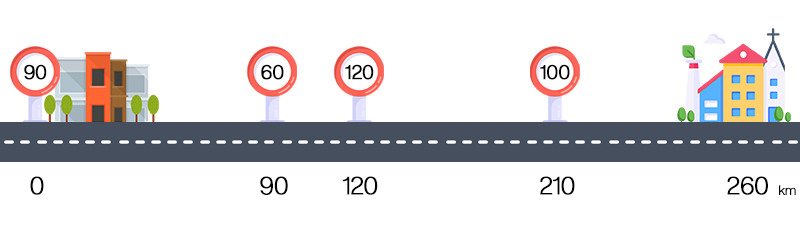
\includegraphics[width = \linewidth]{img/highway.png}
\end{center}

For example, assume we have $n=4$ and $L=260$ as the figure shown above. Then, it will take at least $\frac{90-0}{90}+\frac{120-90}{60}+\frac{210-120}{120}+\frac{260-210}{100}=2.75$ hours to travel from Alpha Town to Beta City under these speed limits.

In order to improve the traffic efficiency, the highway administration department decides to remove some speed-limit signs along the highway. However, due to the traffic restrictions of Alpha Town, the first sign at the origin $x_1=0$ cannot be removed.

Please come up with a dynamic programming algorithm to \textbf{minimize the travel time} from Alpha Town to Beta City by removing no more than $K$ speed-limit signs.

\vspace{0.2in}

\begin{parts}
	\part[2] Define your subproblem for this question.
	\begin{solution}
		%%%%%%%%%%%%%%%%%%%%%%%%%%%%%%%%%%%%%%%%%%%%%%%%%%
		%  Replace the `vspace{2.0in}' with your answer.  
		%%%%%%%%%%%%%%%%%%%%%%%%%%%%%%%%%%%%%%%%%%%%%%%%%%
		% \vspace{2.0in}
		\\let $dp[i][j]$ be the minimal time we will take from $x_1 = 0$ to the $x_i$,
		and the $i$-th sign is remained, $j$ speed-limit signs in the first $i$ signs are removed.\\
		% \\let $dp[i][j][k]$ be the minimal time we will remove some of the signs of $1,2,\cdots,i$,
		% and at most removed $j$ speed-limit signs,
		% and the consecutive $k$ signs are removed start from the $i$-th sign and to its forward.\\
	\end{solution}

    \newpage

	\part[5] Give your Bellman equation to solve the subproblems.
	\begin{solution}
		%%%%%%%%%%%%%%%%%%%%%%%%%%%%%%%%%%%%%%%%%%%%%%%%%%
		%  Replace the `vspace{3.0in}' with your answer.  
		%%%%%%%%%%%%%%%%%%%%%%%%%%%%%%%%%%%%%%%%%%%%%%%%%%
		% \vspace{3.0in}
		\\let $x_{n+1}=L$\\
		$1\leq i\leq n+1; j < i;  j\leq K$\\\\
		$dp[i][j]=min\{dp[k][j-(i-k-1)]+\frac{x_i-x_k}{v_k}\},k=(i-j-1),\cdots,i-1$\\
		% $dp[i][j][0]=min\{dp[i-1][j][k]+\frac{x_{i+1}-x_{i}}{v_{i}}\}$$,(k\leq j)$\\
		% $dp[i][j][k]=min\{dp[i-1][j-1][k-1]+\frac{x_{i+1}-x_{i}}{v_{i-k+1}}\}$$,(1\leq k\leq j)$\\
		\paragraph{Explanation:}
		\begin{itemize}
			% \item if $k\neq 0$,it means that the we will remove the $(i-k+1),\cdots,i$-th signs, 
			% \item if $k=0$, it means that 
			
			%$i$-th sign is not removed. So the following interval will at the speed of $v_i$.
			% \item the following line means that we will remove the $i$-th sign. Since it is consecutive $k$ signs are removed, so the following interval will at the speed of before, i.e. $v_{i-k+1}$.
			% \item $dp[i][j][0]$ means that the $i$-th sign is not removed. So the following interval will at the speed of $v_i$.
			% \item the following line means that we will remove the $i$-th sign. Since it is consecutive $k$ signs are removed, so the following interval will at the speed of before, i.e. $v_{i−k+1}$.
			\item since the $i$-th sign is not removed, so $j<i$.
			\item $k$ means that from the $k+1$-th sign to the $i-1$-th sign are all removed, and the $k$-th sign and the $i$-th sign are remained,
			so there are totally $i-1-k$ signs are removed, so it should transform from $dp[k][j-(i-k-1)]$, and during the period of $x_k$ to $x_i$,
			the limit speed if $v_k$.
			\item since we removed $i-k-1$ signs this time, so $i-k-1\leq j$, $i.e. k\geq i-j-1$
			
		\end{itemize}
	\end{solution}

	\part[2] What is the answer to this question in terms of the subproblems?
	\begin{solution}
		%%%%%%%%%%%%%%%%%%%%%%%%%%%%%%%%%%%%%%%%%%%%%%%%%%
		%  Replace the `vspace{1.5in}' with your answer.  
		%%%%%%%%%%%%%%%%%%%%%%%%%%%%%%%%%%%%%%%%%%%%%%%%%%
		% \vspace{1.5in}
		% \\$min\{dp[n][K][i],i=0,1,\cdots,K\}$\\
		\\$min\{dp[n+1][i],i=0,1,\cdots,K\}$\\
	\end{solution}

	\part[1] What is the runtime complexity of your algorithm?
	\begin{solution}
		%%%%%%%%%%%%%%%%%%%%%%%%%%%%%%%%%%%%%%%%%%%%%%%%%%
		%  Replace the `vspace{1.0in}' with your answer.  
		%%%%%%%%%%%%%%%%%%%%%%%%%%%%%%%%%%%%%%%%%%%%%%%%%%
		% \vspace{1.0in}
		\\$\Theta(nk^2)$\\
	\end{solution}
\end{parts}

	\newpage

	\titledquestion{Pairwise DNA Sequence Alignment}

Given two DNA sequences: a query sequence $Q=\langle Q_1, \dots, Q_m\rangle$ of $m$ nucleotides and a subject sequence $S=\langle S_1, \dots, S_n\rangle$ of $n$ nucleotides. There are $4$ types of nucleotides, namely Adenine (A), Cytosine (C), Guanine (G) and Thymine (T). We provide a scoring matrix for nucleotides at the same index of these two sequences:

\begin{table}[!htbp]
	\centering
	\begin{tabular}{|c|c|c|c|c|} \hline
		  & A  & C  & G  & T  \\ \hline
		A & 1  & -5 & -1 & -5 \\ \hline
		C & -5 & 1  & -5 & -1 \\ \hline
		G & -1 & -5 & 1  & -5 \\ \hline
		T & -5 & -1 & -5 & 1  \\ \hline
	\end{tabular}
\end{table}

where $\text{Score}(X, X)$ on the diagonal represents the score of a successful match for nucleotide $X$ at the same index of both sequences and  $\text{Score}(X, Y)$ indicates the penalty for mismatching nucleotide $X$ by nucleotide $Y$.

For example, assume we have $m=n$ here and there are two sequences $Q=\langle TGGTG\rangle$ and $S=\langle ATCGT\rangle$. Then the alignment score for these two sequences is
\[
	\begin{aligned}
		\text{Score}(Q, S) & = \sum_{i}^{n} \text{Score}(Q_i, S_i) \\
		                   & = \text{Score}(T, A)+\text{Score}(G, T)+\text{Score}(G, C)+\text{Score}(T, G)+\text{Score}(G, T) \\
		                   & = (-5)+(-5)+(-5)+(-5)+(-5) \\
		                   & = -25
	\end{aligned}
\]

However, if $m \neq n$, we must insert several gaps `$-$' to make two sequences the same length. What's more, in order to align two sequences for higher score, we can also insert arbitrary number of gaps `$-$' to each sequence at arbitrary index. However, adding one gap will result in a gap penalty $\text{Penalty}(X, -)=\text{Penalty}(-, Y)=-2$.

Assume after inserting $4$ gaps, we obtain $Q^\prime=\langle -T-GGTG\rangle$ and $S^\prime=\langle ATCG-T-\rangle$. Then the recomputed alignment score is:
\[
	\begin{aligned}
		\text{Score}(Q^\prime, S^\prime) & = \text{Penalty}(-, A) +\text{Score}(T, T)+\text{Penalty}(-, C) + \text{Score}(G, G) \\
		                                 & \ \ \  +\text{Penalty}(G, -)+\text{Score}(T, T)+ \text{Penalty}(G, -)               \\
		                                 & = (-2)+1+(-2)+1+(-2)+1+(-2)                                                          \\
		                                 & = -5
	\end{aligned}
\]
Notice that $Q^\prime$ and $S^\prime$ should share the same length after inserting gaps.

Given the scoring matrix and gap penalty, please come up with a dynamic programming algorithm to \textbf{maximize the pairwise alignment score} of a pair of DNA sequences by inserting gaps to these two sequences.

\newpage
\begin{parts}
	\part[2] Define your subproblem for this question.
	\begin{solution}
		%%%%%%%%%%%%%%%%%%%%%%%%%%%%%%%%%%%%%%%%%%%%%%%%%%
		%  Replace the `vspace{1.5in}' with your answer.  
		%%%%%%%%%%%%%%%%%%%%%%%%%%%%%%%%%%%%%%%%%%%%%%%%%%
		% \vspace{1.5in}
		let $dp[i][j]$ means that the maximum value we can get when matching the first $i$ nucleotides of $Q$, and the first $j$ nucleotides of $S$.\\
		suppose that the two sequence's index start from $1$.\\
	\end{solution}

	\part[5] Give your Bellman equation to solve the subproblems.
	\begin{solution}
		%%%%%%%%%%%%%%%%%%%%%%%%%%%%%%%%%%%%%%%%%%%%%%%%%%
		%  Replace the `vspace{1.5in}' with your answer.  
		%%%%%%%%%%%%%%%%%%%%%%%%%%%%%%%%%%%%%%%%%%%%%%%%%%
		% \vspace{1.5in}
		\\$dp[0][0]=0$\\
		\\$dp[i][j] = max\{$\\
		$dp[i-1][j-1]+Score(Q[i],S[j]),$\\
		$dp[i-1][j]+Penalty(Q[i],-),$\\
		$dp[i][j-1]+Penalty(-,S[j])$\\
		$\}   (i > 0, j > 0)$\\
		\paragraph{Explanation:}
		\begin{itemize}
			\item The $1$st term in $\max$: do not use $"-"$, just take the last untaken nucleotide, so $Q_i$ and $S_j$ are matched.
			\item The $2$nd term in $\max$: we will use the $"-"$ on $S$, so $Q_i$ will match $"-"$.
			\item The $3$rd term in $\max$: we will use the $"-"$ on $Q$, so $S_j$ will match $"-"$.
		\end{itemize}

	\end{solution}

	\part[2] What is the answer to this question in terms of the subproblems?
	\begin{solution}
		%%%%%%%%%%%%%%%%%%%%%%%%%%%%%%%%%%%%%%%%%%%%%%%%%%
		%  Replace the `vspace{1.5in}' with your answer.  
		%%%%%%%%%%%%%%%%%%%%%%%%%%%%%%%%%%%%%%%%%%%%%%%%%%
		% \vspace{1.5in}
		\\$dp[n][m]$\\
		$n$ is the length of $Q$, while $m$ is the length of $S$.\\
	\end{solution}

	\part[1] What is the runtime complexity of your algorithm?
	\begin{solution}
		%%%%%%%%%%%%%%%%%%%%%%%%%%%%%%%%%%%%%%%%%%%%%%%%%%
		%  Replace the `vspace{1.0in}' with your answer.  
		%%%%%%%%%%%%%%%%%%%%%%%%%%%%%%%%%%%%%%%%%%%%%%%%%%
		% \vspace{1.0in}
		\\$\Theta(nm)$\\
		$n$ is the length of $Q$, while $m$ is the length of $S$.\\
	\end{solution}
\end{parts}

\end{questions}

\end{document}